%!TEX root = karen.tex

\chapter{Numerical Validation} 

\label{sec:validation}

Here, we present the first results in the literature for parallelizing RBF-FDs on multi-CPU and multi-GPU architectures for solving PDEs. 
 To verify our multi-CPU, single GPU and multi-GPU implementations, two hyperbolic PDEs on the surface of the sphere are tested: 1) vortex roll-up \cite{NairTransport05, NairJablonowski08} and 2) solid body rotation \cite{JakobChien1995}. These tests were chosen since they are not only standard in the numerical literature, but also
for the development of RBFs in solving PDEs on the sphere \cite{FlyerWright07, Fornberg2008, FlyerLehto10, Fornberg2011a}. Although any `approximately evenly' distributed nodes on the sphere would suffice for our purposes, maximum determinant (MD) node distributions on the sphere are used (see \cite{Sloan2003} for details) in order to be consistent with previously published results (see e.g., \cite{FlyerWright07} and \cite{FornbergLehto11}). Node sets from 1024 to 27,556 are considered with stencil sizes ranging from 17 to 101.

All results in this section are produced by the single-GPU implementation. Multi-CPU and multi-GPU implementations are verified to produce these same results. Synchronization of the solution at each time-step and the use of double precision on both the CPU and GPU ensure consistent results regardless of the number and/or choice of CPU vs GPU. Eigenvalues are computed on the CPU by the Armadillo library \cite{armadillo2010}.


\subsection{Vortex Rollup}
\label{sec:numerical_validation}
The first test case demonstrates vortex roll-up of a fluid on the surface of a unit sphere. An angular velocity field causes the initial condition to spin into two diametrically opposed but stationary vortices.

The governing PDE in latitude-longitude coordinates, $(\theta,\lambda)$, is
\begin{equation}
\pd{h}{t} + \frac{u}{\cos \theta} \pd{h}{\lambda} = 0
\label{eq:vortex}
\end{equation}
where the velocity field, $u$, only depends on latitude and is given by
\begin{equation*}
u  = \omega(\theta) \cos \theta.
\end{equation*}
Note that the $\cos \theta$ in $u$ and $1/\cos{\theta}$ in (\ref{eq:vortex}) cancel in the analytic formulation, so the discrete operator approximates $\omega(\theta) \pd{}{\lambda}$. 

Here, $\omega(\theta)$ is the angular velocity component given by
\begin{equation*}
\omega(\theta) =
\begin{cases}
\frac{3\sqrt{3}}{2 \rho(\theta)} \mathrm{sech}^{2}(\rho(\theta)) \mathrm{tanh}(\rho(\theta)) & \rho(\theta) \neq 0 \\
0 & \rho(\theta) = 0
\end{cases}
\end{equation*}
where $\rho(\theta) = \rho_0 \cos \theta$ is the radial distance of the vortex with $\rho_0=3$. The exact solution to (\ref{eq:vortex}) at non-dimensional time $t$ is
\begin{equation*}
h(\lambda, \theta, t) = 1 - \mathrm{tanh}\left( \frac{\rho(\theta)}{\gamma} \sin(\lambda - \omega(\theta) t) \right),
\end{equation*}
where $\gamma$ defines the width of the frontal zone.

From a method of lines approach, the discretized version of (\ref{eq:vortex}) is
\begin{equation}
%\pd{\mathbf{h}}{t} = - \text{diag}(\omega(\theta)) D_\lambda \mathbf{h}.
\d{\mathbf{h}}{t} = - \text{diag}(\omega(\theta)) D_\lambda \mathbf{h}.
\label{eq:vortex_matrix_form}
\end{equation}
where $D_\lambda$ is the DM containing the RBF-FD weights that approximate $\pd{}{\lambda}$ at each node on the sphere.

For stability, hyperviscosity is added to the right hand side of (\ref{eq:vortex_matrix_form}) in the form given in (\ref{eq:evaluation_with_hyperviscosity}). The scaling parameter $\gamma_c$ and the order of hyperviscosity $k$ are given in
Table~\ref{tbl:vortex_hv_params}. The goal when choosing $k$ is to damp the higher spurious eigenmodes of $\text{diag}(\omega(\theta)) D_\lambda$ while leaving the lower physical modes that can be resolved by the stencil intact. In this process, the eigenvalues will be pushed into the left half of the complex plane. Then, $\gamma_c$ is used to condense the eigenvalues as near to the imaginary axis as possible. Figure \ref{fig:vortex_eigs_hv} shows the effect of hyperviscosity on the eigenvalues of the DM, $-diag(\omega(\theta)) D_\lambda$, in (\ref{eq:vortex_matrix_form}). 

In order to scale to large node sets, the RBF shape parameter, $\epsilon$, is chosen such that the mean condition number of the local RBF interpolation matrices $\bar{\kappa}_A = \frac{1}{N}\sum_{j=1}^N (\kappa_A)_j$ is kept constant as $N$ increases ($(\kappa_A)_j$ is the condition number of the interpolation matrix in (\ref{syst}), representing the $j^{th}$ stencil). For a constant mean condition number, $\epsilon$ varies linearly with $\sqrt{N}$ (see \cite{FlyerLehto11} Figure 4a and b). This is not surprising since the condition number strongly depends on the quantity $\epsilon r$, where $r\thicksim1/\sqrt{N}$ on the sphere. Thus, to obtain a constant condition number, we let $\epsilon (N) = c_1 \sqrt{N} - c_2$, where $c_1$ and $c_2$ are constants based on \cite{FlyerLehto11}.

\begin{table}[t]
\caption{Values for hyperviscosity and the RBF shape parameter $\epsilon$ for vortex roll-up test.}
\begin{center}
\begin{tabular}{|c|c|c|c|c|c|}
\hline		     & \multicolumn{2}{c|}{$\epsilon = c_1 \sqrt{N} - c_2$} & \multicolumn{2}{c|}{$H = -\gamma_{c} N^{-k} \Delta^{k}$ } \\ \hline
Stencil Size ($n$) & $c_{1}$ & $c_{2}$ & $k$ & $\gamma_c$ \\ \hline
17 & 0.026 & 0.08 & 2 & $8$ \\
31 & 0.035 & 0.1  & 4 & $800$ \\
50 & 0.044 & 0.14 & 4 & $145$ \\
101 & 0.058 & 0.16 & 4 & $40$ \\ \hline
\end{tabular}
\end{center}
\label{tbl:vortex_hv_params}
\end{table}



\begin{figure}[htb]
\begin{center}
\subfigure[No Hyperviscosity]
{
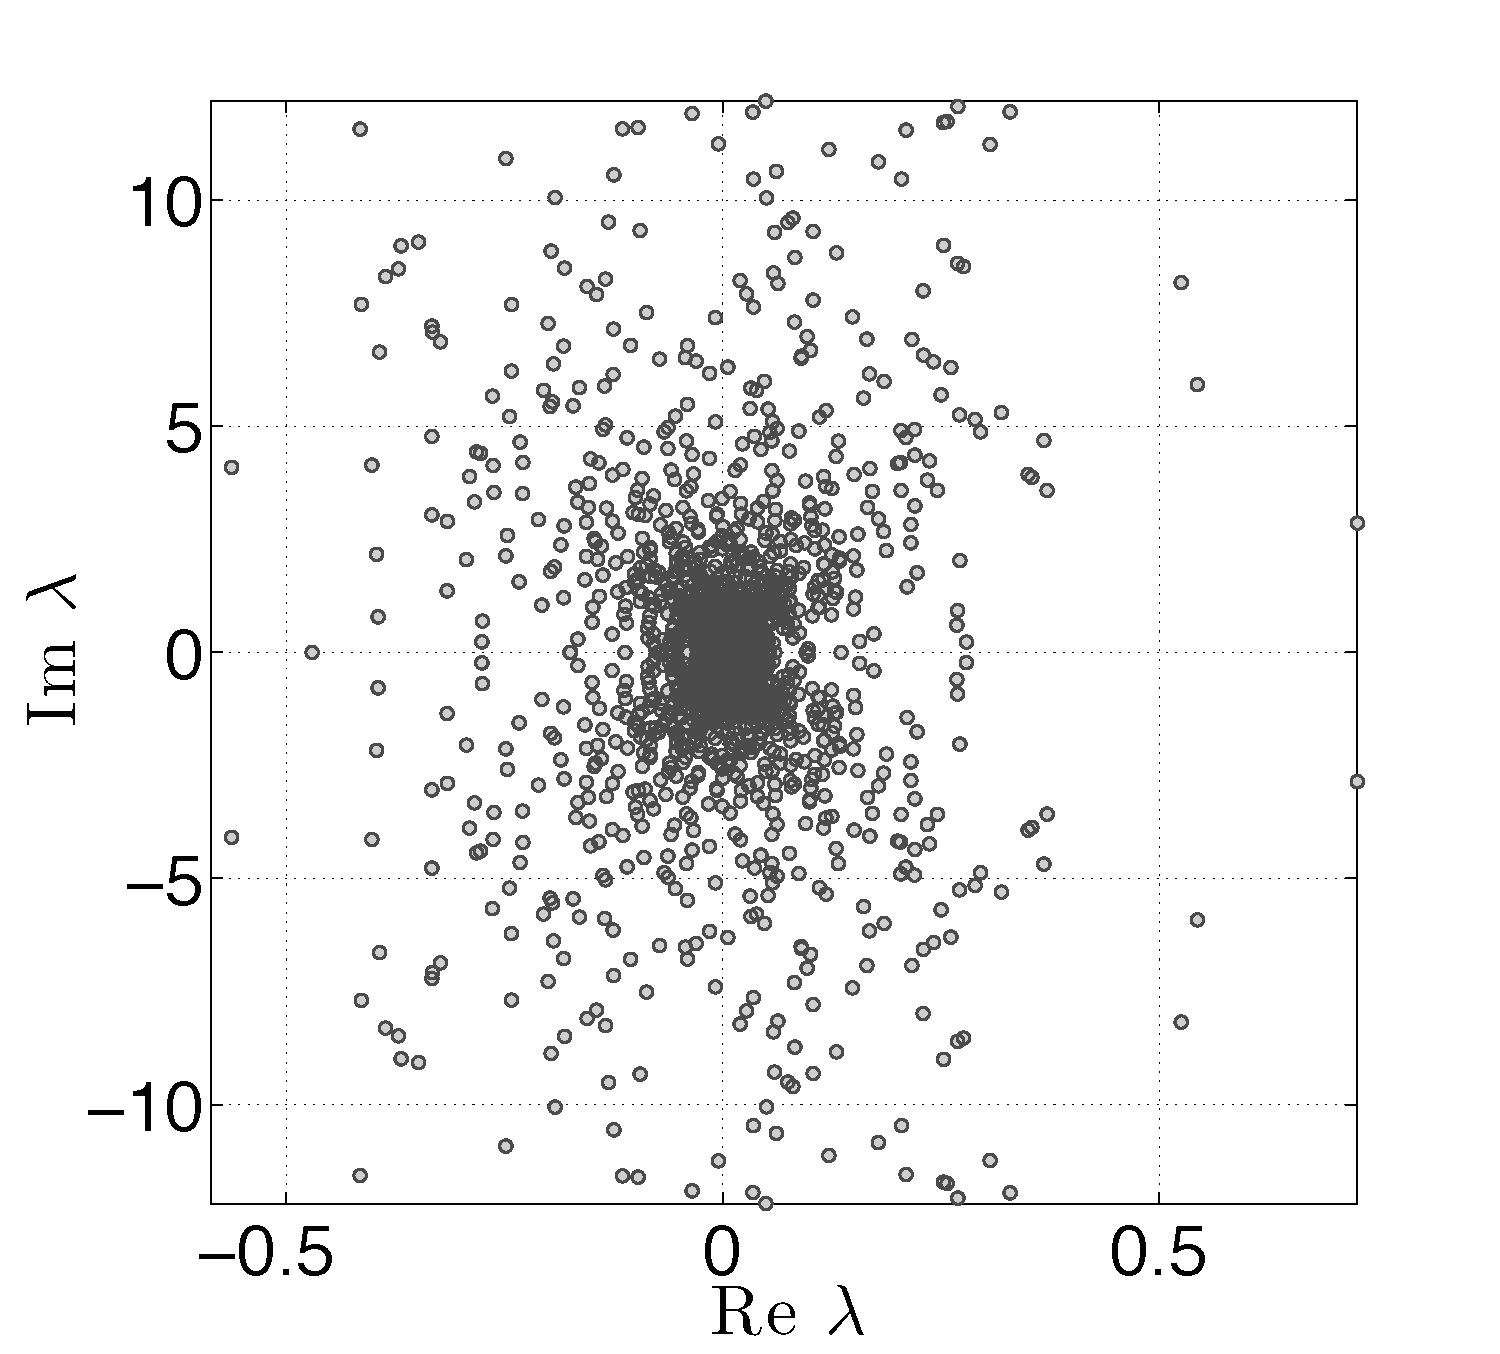
\includegraphics[width=2.85in]{figures/paper1/figures/vortex_rollup/eigs_N4096_n101_noHV.pdf}
\label{fig:vortex_eigs_nohv}
}
\subfigure[With Hyperviscosity]
{
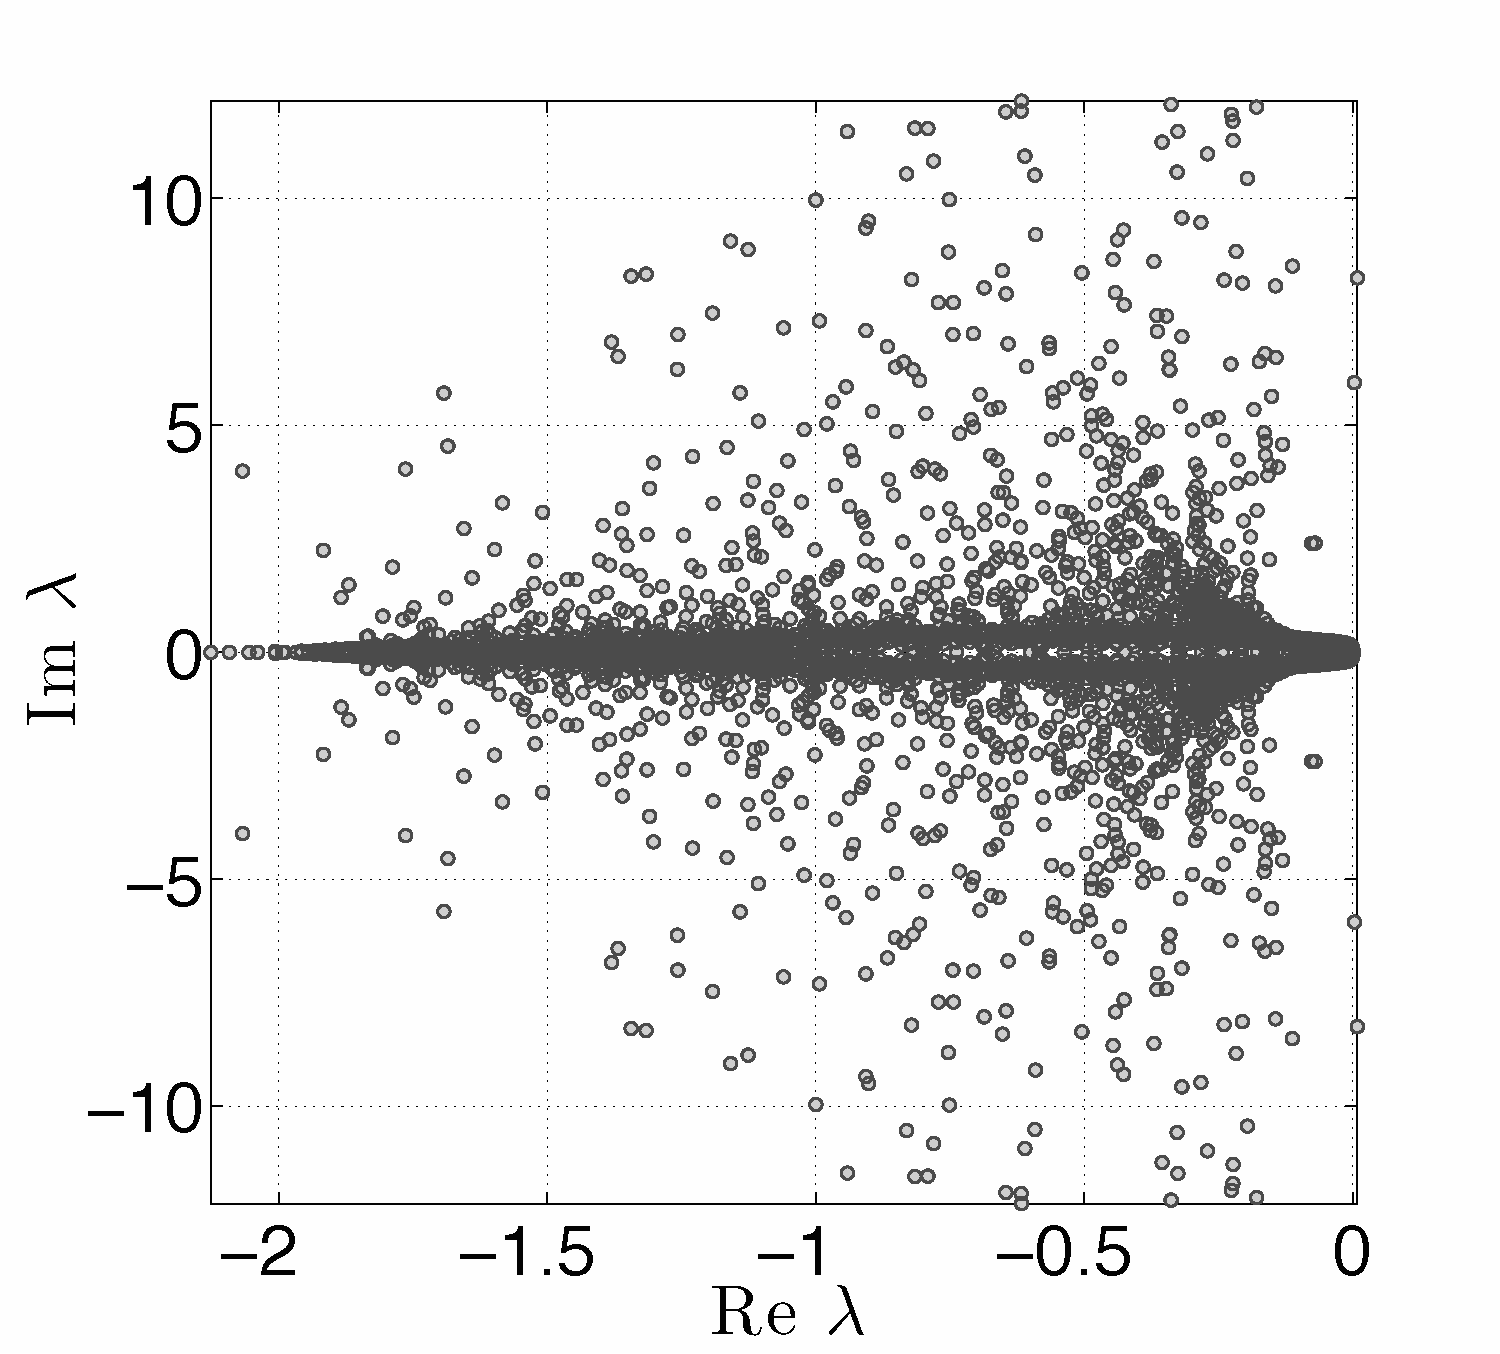
\includegraphics[width=2.85in]{figures/paper1/figures/vortex_rollup/eigs_N4096_n101_HV_k4_gamma40.pdf}
\label{fig:vortex_eigs_hv}
}
\caption{Eigenvalues of $\text{diag}(\omega(\theta)) D_\lambda$ for the vortex roll-up test case for $N=4096$ nodes, stencil size $n=101$ and $\epsilon = 3.5$. Left: no hyperviscosity. Right: hyperviscosity enabled with $k=4$ and $\gamma_c = 40$.
}
\label{fig:eig_vortex}
\end{center}
\end{figure}

\begin{figure}[htbp]
\begin{center}
\subfigure[Computed Solution]
{
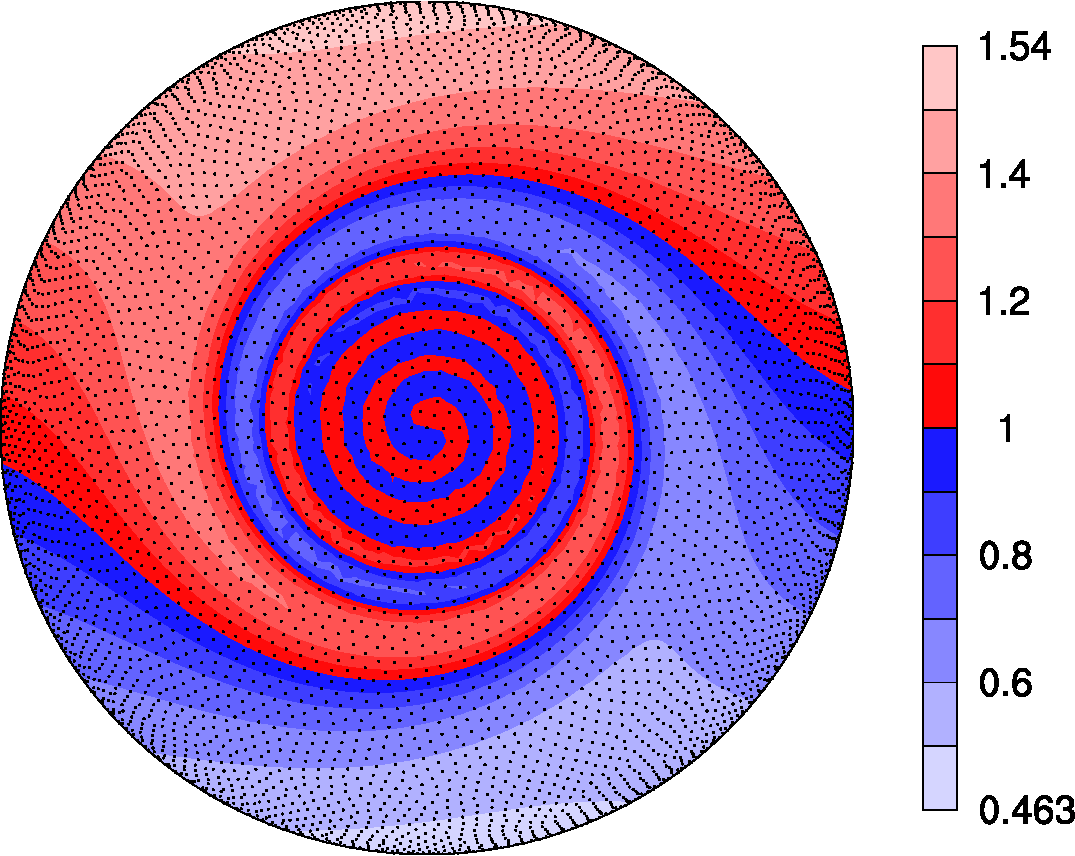
\includegraphics[width=2.5in]{figures/paper1/figures/vortex_rollup/vortexComputedSolution-eps-converted-to.pdf}
\label{fig:vortex_approx}
}
\subfigure[Relative Absolute Error ]
{
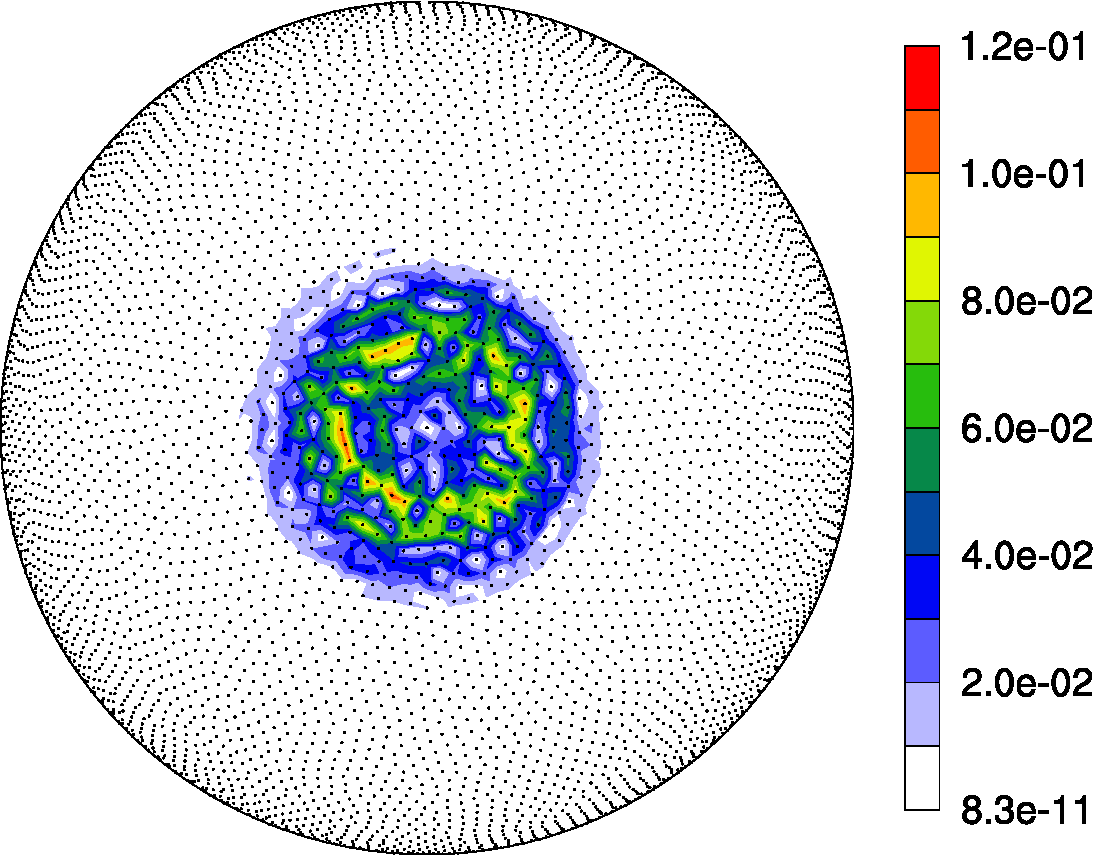
\includegraphics[width=2.5in]{figures/paper1/figures/vortex_rollup/vortexRelativeError-eps-converted-to.pdf}
\label{fig:vortex_relerr}
}
\caption{Vortex roll-up solution at time $t=10$ using RBF-FD with $N=10,201$ and $n=50$ point stencil. Normalized $\ell_2$ error of solution at $t=10$ is $1.25(10^{-2})$ }
\label{fig:vortex_t10}
\end{center}
\end{figure}

Figure~\ref{fig:vortex_t10} shows the solution to Equation~(\ref{eq:vortex}) at $t = 10$, on $N=10201$ nodes, with stencil size $n=50$. This resolution is sufficient to properly capture the vortices at $t=10$, but lower resolutions would suffer approximation errors associated with insufficient grid resolution. 
For this reason, the solution at $t=3$ is considered in the normalized $\ell_2$ error convergence study presented in Figure~\ref{fig:conv_plot_vortex_hv}. The time step $\Delta t = 0.05$ for all resolutions.

\begin{figure}[htbp!]
\begin{center}
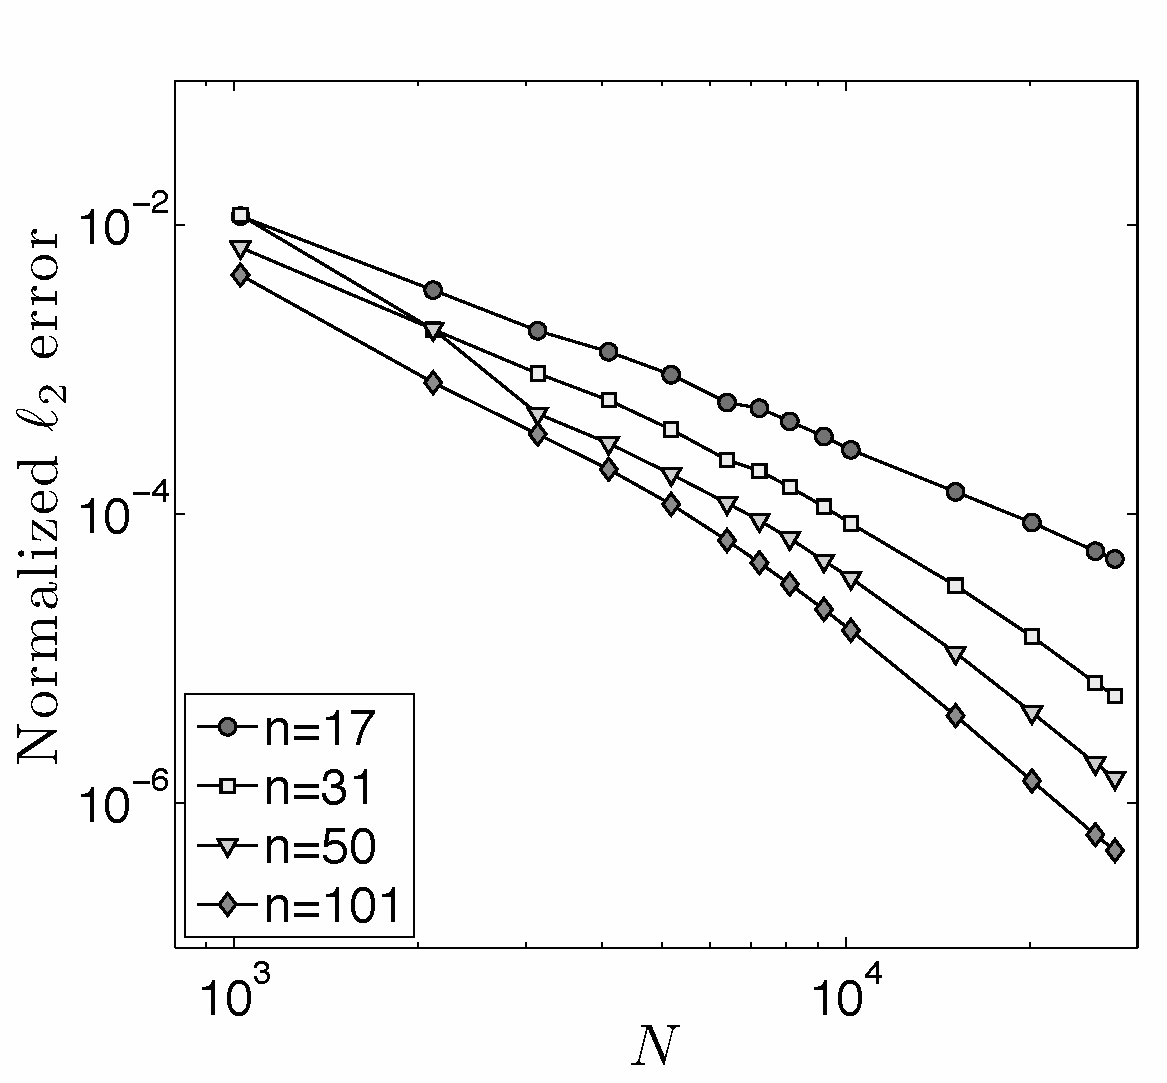
\includegraphics[width=3in] {figures/paper1/figures/vortex_rollup/convergence_plot_hv.pdf}
\caption{Convergence plot for vortex roll-up at $t=3$. }
\label{fig:conv_plot_vortex_hv}
\end{center}
\end{figure}

\subsection{Solid body rotation}

The second test case simulates the advection of a cosine bell over the surface of a unit sphere at an angle $\alpha$ relative to the pole of a standard latitude-longitude grid. The governing PDE is
\begin{equation}
\pd{h}{t} + \frac{u}{\cos \theta} \pd{h}{\lambda} + v \pd{h}{\theta} = 0, \label{eq:cosine_bell}
\end{equation}
with velocity field,
\begin{equation*}
%\begin{cases}
%u =  \cos \theta \cos \alpha + \sin \theta \cos \lambda \sin \alpha,  & \\
%v =  -\sin \lambda \sin \alpha &.
%\end{cases}
\begin{cases}
u =  u_0 (\cos \theta \cos \alpha + \sin \theta \cos \lambda \sin \alpha),  & \\
v =  -u_0(\sin \lambda \sin \alpha) &.
\end{cases}
\end{equation*}
inclined at an angle $\alpha$ relative to the polar axis and velocity $u_0 = 2 \pi / (1036800$ seconds$)$ to require 12 days per revolution of the bell as in \cite{NairTransport05, FlyerWright07}.
%$u_0 = 1$.

The discretized form of (\ref{eq:cosine_bell}) is
\begin{equation}
%D = \text{diag}(\frac{u}{\cos \theta}) D_\lambda + \text{diag}(v) D_\theta
\d{\mathbf{h}}{t} = -\text{diag}\left(\frac{u}{\cos \theta}\right) D_\lambda \mathbf{h} - \text{diag}(v) D_\theta \mathbf{h}
\label{eq:cosine_with_hyperviscosity}
\end{equation}
where DMs $D_\lambda$ and $D_\theta$ contain RBF-FD weights corresponding to all $N$ stencils that approximate $\pd{}{\lambda}$ and $\pd{}{\theta}$ respectively. Rather than merge the differentiation matrices in (\ref{eq:cosine_with_hyperviscosity}) into one operator, our implementation evaluates them as two sparse matrix-vector multiplies. The separate matrix-vector multiplies are motivated by an effort to provide general and reusable GPU kernels. Additionally, they artificially increase the amount of computation compared to the vortex roll-up test case to simulate cases when operators cannot be merged into one DM (e.g., a non-linear PDE).

By splitting the DM, the singularities at the poles ($1 / \cos{\theta} \rightarrow \infty$ as $\theta \rightarrow \pm\frac{\pi}{2}$) in (\ref{eq:cosine_bell}) remain. However, in this case, the approach functions without amplification of errors because the MD node sets have nodes near, but not on, the poles. As noted in \cite{FlyerWright07, FornbergLehto11}, applying the entire spatial operator to the right hand side of Equation~\ref{syst} generates a single DM that analytically removes the singularities at poles. 

We will advect a $C^1$ cosine bell height-field given by
\begin{equation*}
h  =
\begin{cases}
\frac{h_0}{2} (1 + \cos(\frac{\pi \rho}{R}))  & \rho \le R  \\
 0 &  \rho \geq R
\end{cases}
\end{equation*}
having a maximum height of $h_0 = 1$, a radius $R = \frac{1}{3}$ and centered at $(\lambda_c, \theta_c) = (^{3\pi}/_{2}, 0)$, with 
$\rho = \arccos( \sin \theta_{c} \sin \theta + \cos \theta_{c} \cos \theta \cos (\lambda - \lambda_{c}) )$.
The angle of rotation, $\alpha =\ ^{\pi}/_{2}$, is chosen to transport the bell over the poles of the coordinate system.

\begin{table}[ht!]
\caption{Values for hyperviscosity and RBF shape parameter for the cosine bell test. }
\begin{center}
\begin{tabular}{|c|c|c|c|c|c|}
\hline		     & \multicolumn{2}{c|}{$\epsilon = c_1 \sqrt{N} - c_2$} & \multicolumn{2}{c|}{$H = -\gamma_{c} N^{-k} \Delta^{k}$ } \\ \hline
Stencil Size ($n$) & $c_{1}$ & $c_{2}$ & $k$ & $\gamma_c$ \\ \hline
17 & 0.026 & 0.08 & 2 & $8 * 10^{-4}$ \\
31 & 0.035 & 0.1 & 4 & $5 * 10^{-2}$ \\
50 & 0.044 & 0.14 & 6 & $5 * 10^{-1}$ \\
101 & 0.058 & 0.16 & 8 & $5 * 10^{-2}$ \\ \hline
\end{tabular}
\end{center}
\label{tbl:cos_hv_params}
\end{table}

\begin{figure}[ht!]
\begin{center}
\subfigure[No Hyperviscosity]
{
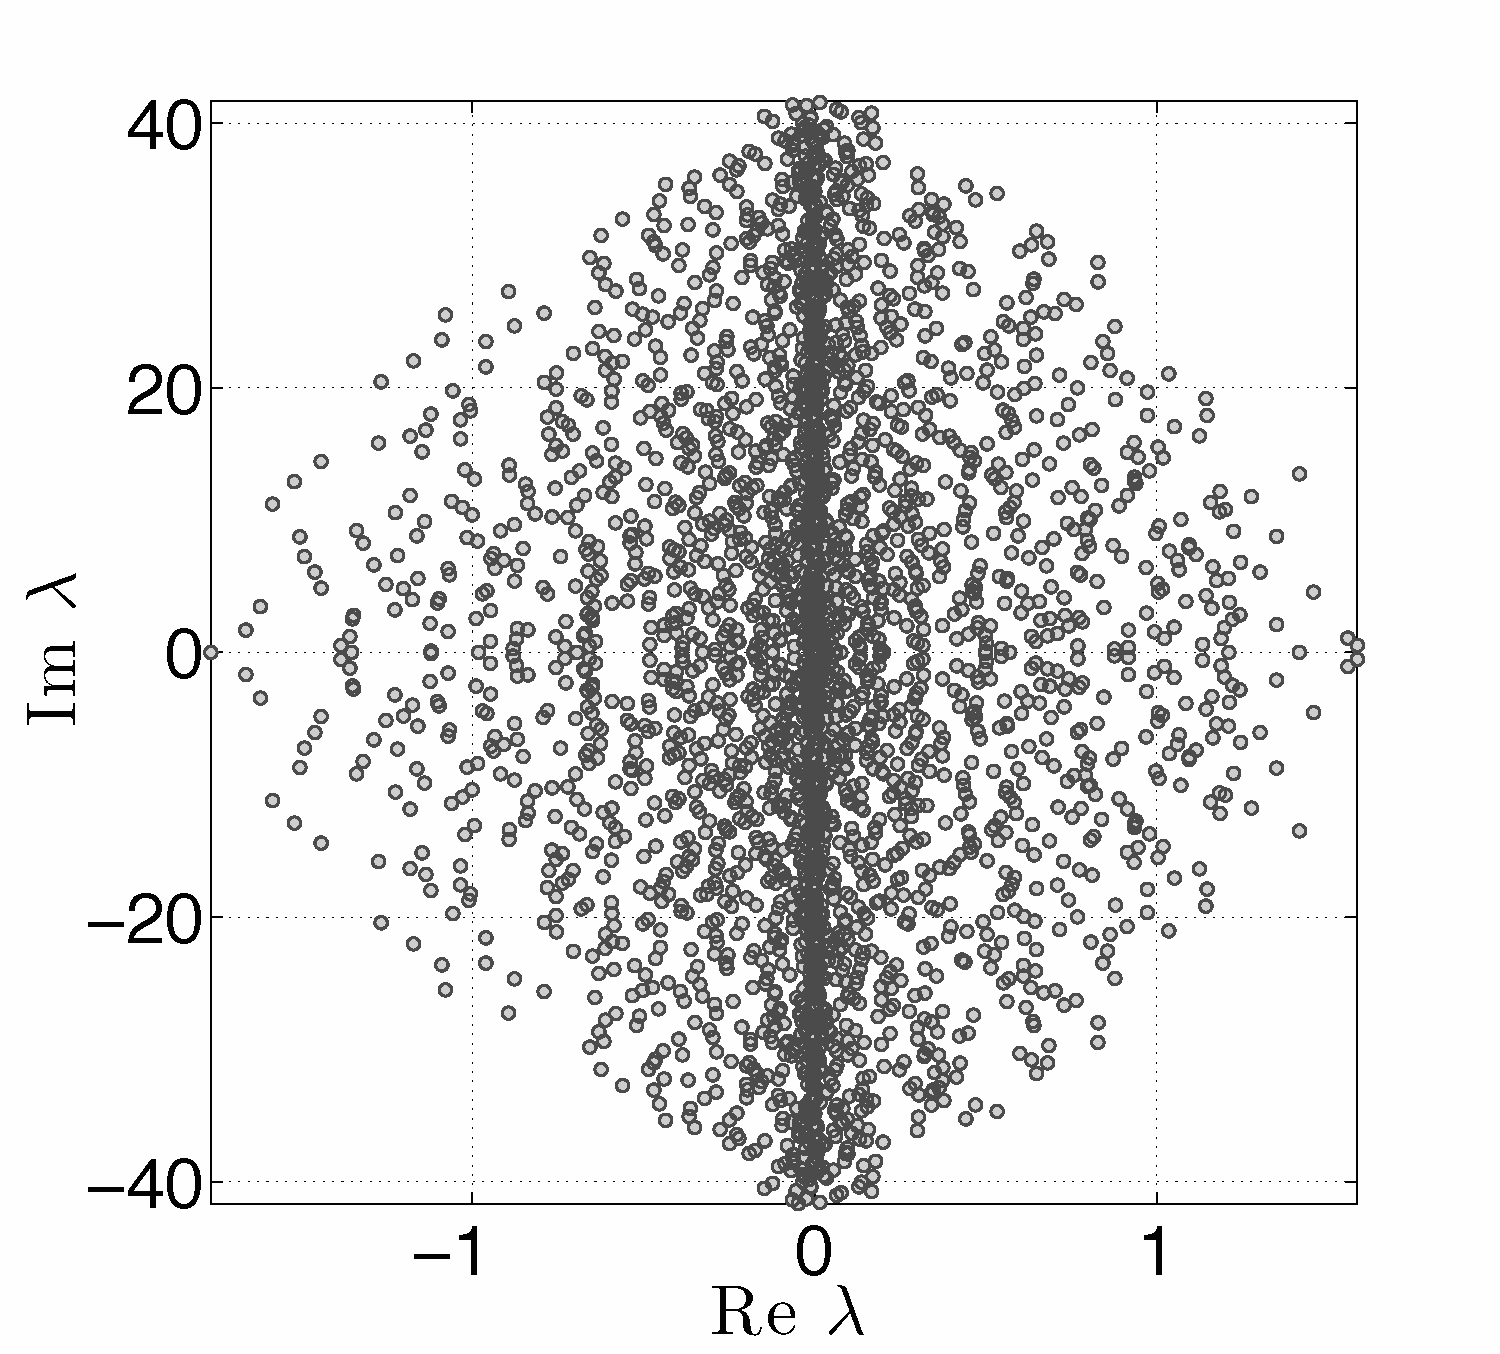
\includegraphics[width=2.75in]{figures/paper1/figures/cosine_bell/eigs_N4096_n101_noHV_SCALED.pdf}
\label{fig:cosine_eigs_nohv}
}
\subfigure[With Hyperviscosity]
{
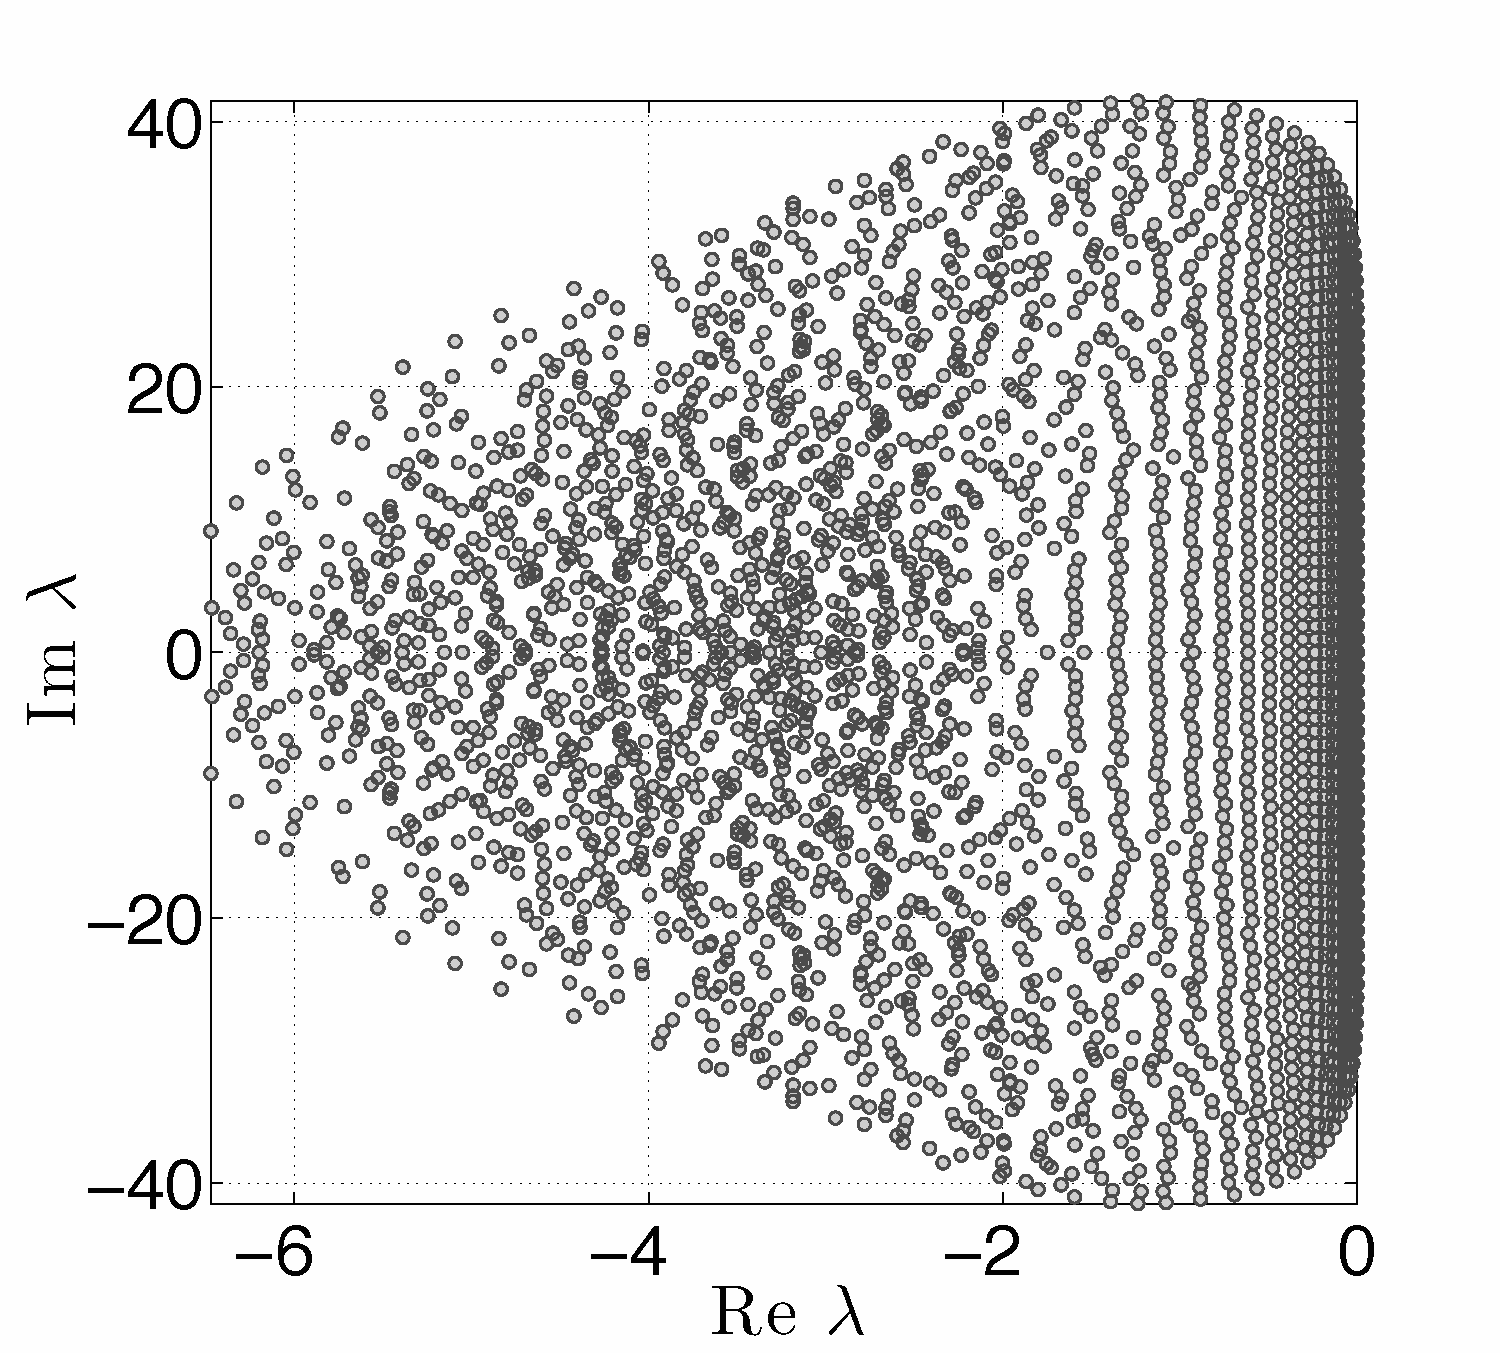
\includegraphics[width=2.75in]{figures/paper1/figures/cosine_bell/eigs_HV_N4096_n101_k8_gamma5e_m2_SCALED.pdf}
\label{fig:cosine_eigs_hv}
}
\caption{Eigenvalues of (\ref{eq:cosine_with_hyperviscosity}) for the cosine bell test case with $N=4096$ nodes, stencil size $n=101$, and $\epsilon = 3.5$. Left: no hyperviscosity. Right: hyperviscosity enabled with $k=8$ and $\gamma_c = 5*10^{-2}$. Eigenvalues are divided by $u_0$ to remove scaling effects of velocity.  
}
\label{fig:eig_cosine}
\end{center}
\end{figure}

\begin{figure}[ht!]
\begin{center}
\subfigure[10 Revolutions]
{
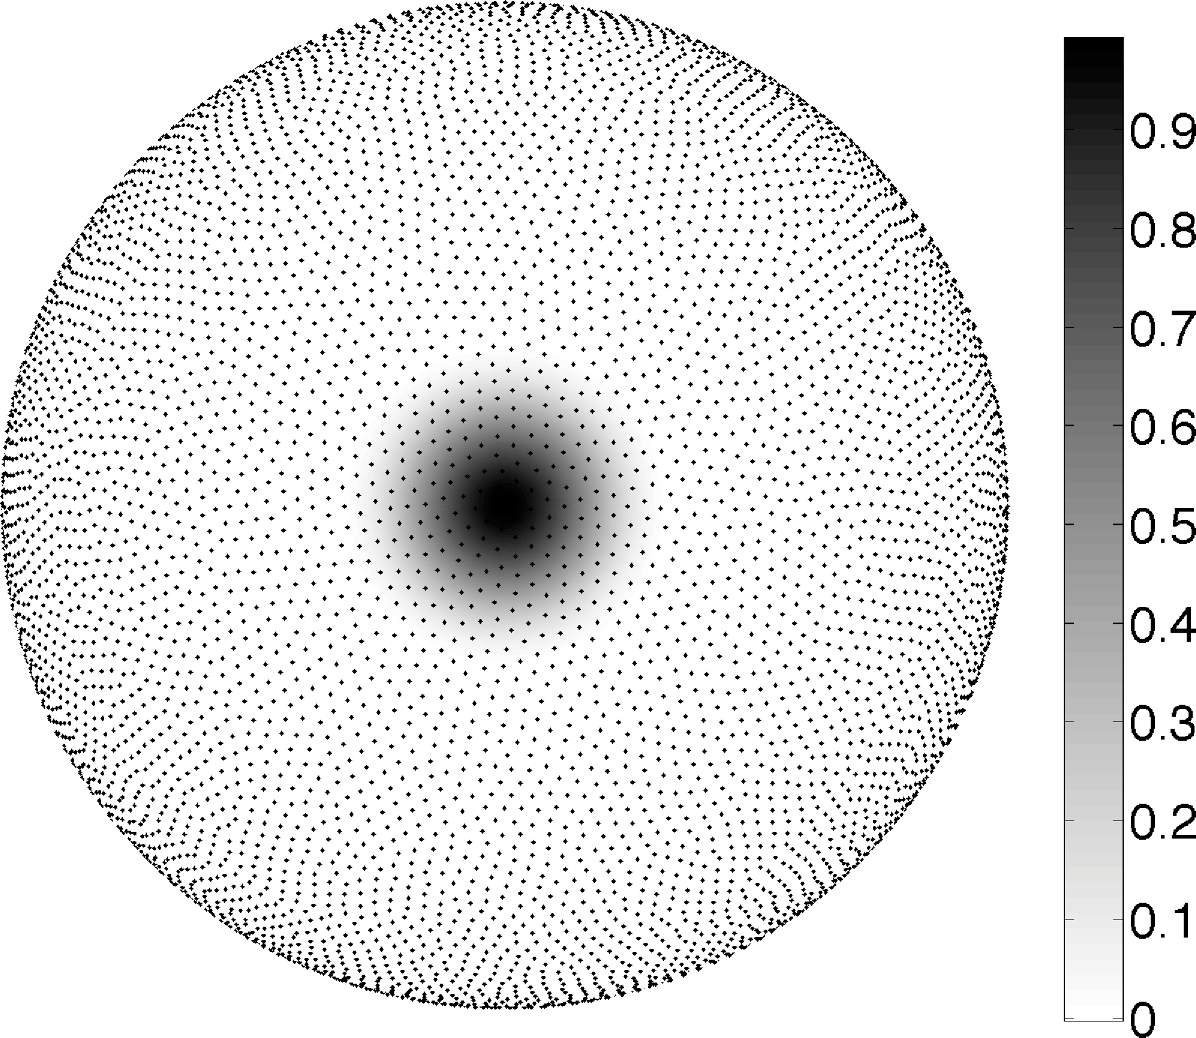
\includegraphics[width=2.4in]{figures/paper1/figures/cosine_bell/trimmed_ComputedSolution_ManualBar.pdf}
\label{fig:cosine_approx}
}
\subfigure[Absolute Error at 10 revolutions]
{
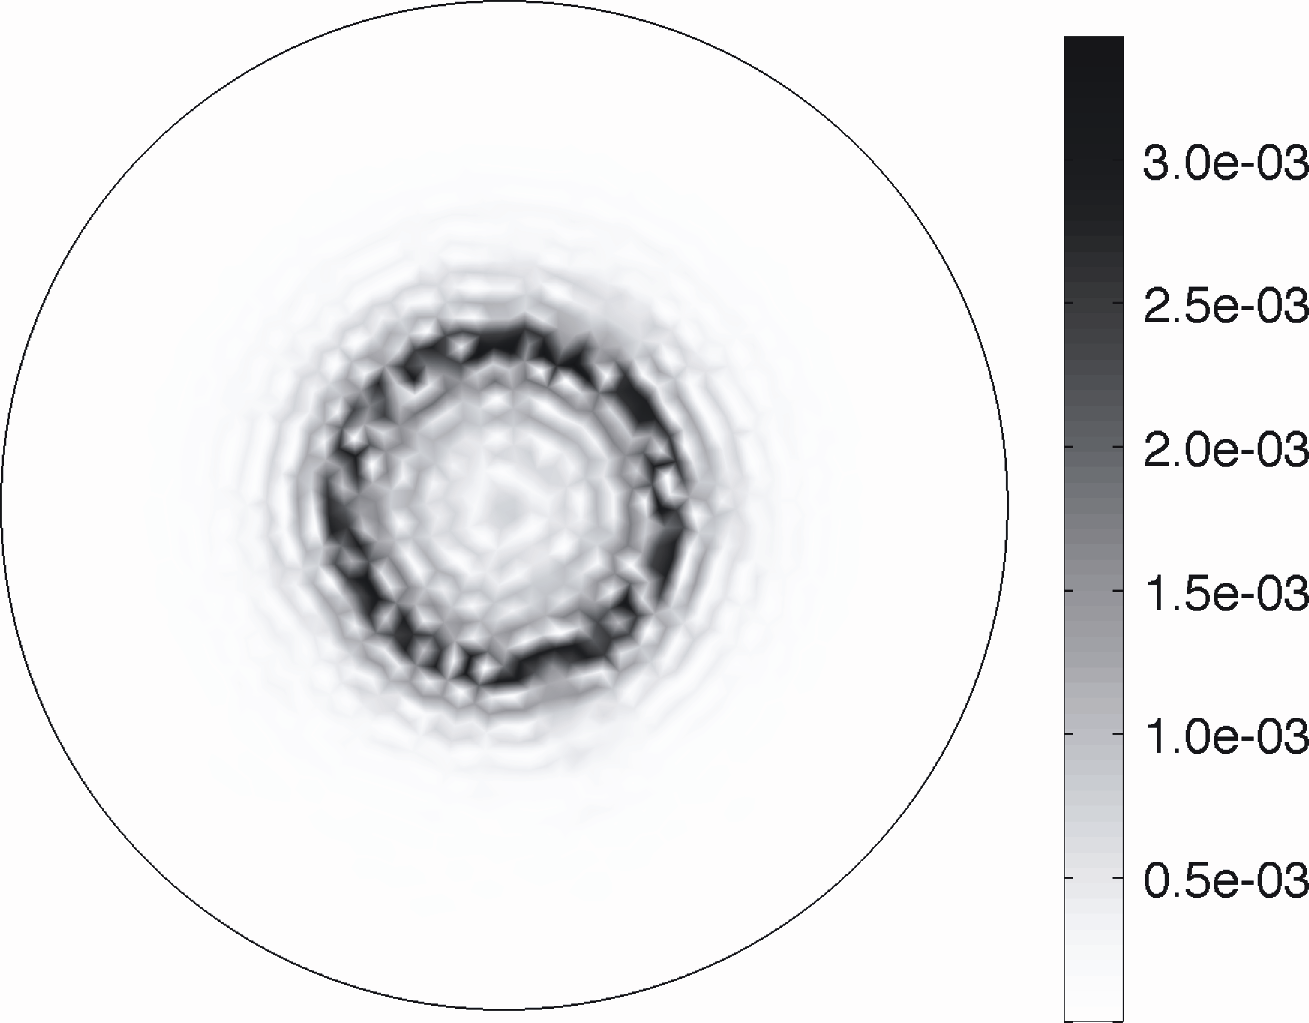
\includegraphics[width=2.6in]{figures/paper1/figures/cosine_bell/trimmed_Error_CoveredScale2.pdf}
\label{fig:cosine_abserror}
}
\caption{Cosine bell solution after 10 revolutions with $N=10201$ nodes and stencil size $n=101$.
Hyperviscosity parameters are $k = 8$, $\gamma_c = 5(10^{-2})$. 
}
 \label{fig:cosine_10revs}
\end{center}
\end{figure}

Figure~\ref{fig:eig_cosine} compares eigenvalues of the DM for $N=4096$ nodes and stencil size $n=101$ before and after hyperviscosity is applied. To avoid scaling effects of velocity on the eigenvalues, they have been scaled by $1/u_0$.  The same approach as in the vortex roll-up case is used to determine the parameters for hyperviscosity and $\epsilon$. Our tuned parameters are presented in 
%\blue{However, note the difference in scale on the real axis compared to the vortex roll-up case; the initial range of the real part of the eigenvalues is approximately four orders of magnitude smaller. In this case, eigenvalues are more sensitive to the hyperviscosity filter. 
Table~\ref{tbl:cos_hv_params}.
% provides appropriate parameters for hyperviscosity in this test case. %, which reflect the difference in scale of $\gamma_c$ compared to Table~\ref{tbl:vortex_hv_params}.
%The parameters for hyperviscosity are dependent on $u_0$ 

%\clearpage

Figure~\ref{fig:cosine_10revs} shows the cosine bell transported ten full revolutions around the sphere. Without hyperviscosity, RBF-FD cannot complete a single revolution of the bell before instability takes over. However, adding hyperviscosity allows computation to extend to dozens or even thousands of revolutions and maintain stability (e.g., see \cite{FornbergLehto11}). After ten revolutions, the cosine bell is still intact. The majority of the absolute error (Figure~\ref{fig:cosine_abserror}) appears at the base of the $C^1$ bell where the discontinuity appears in the derivative. At ten revolutions, Figure~\ref{fig:conv_cosine_bell} illustrates the convergence of the RBF-FD method. All tests in Figure~\ref{fig:conv_cosine_bell} assume 1000 time-steps per revolution (i.e., $\Delta t = 1036.8$ seconds).


\begin{figure}[htbp]
\begin{center}
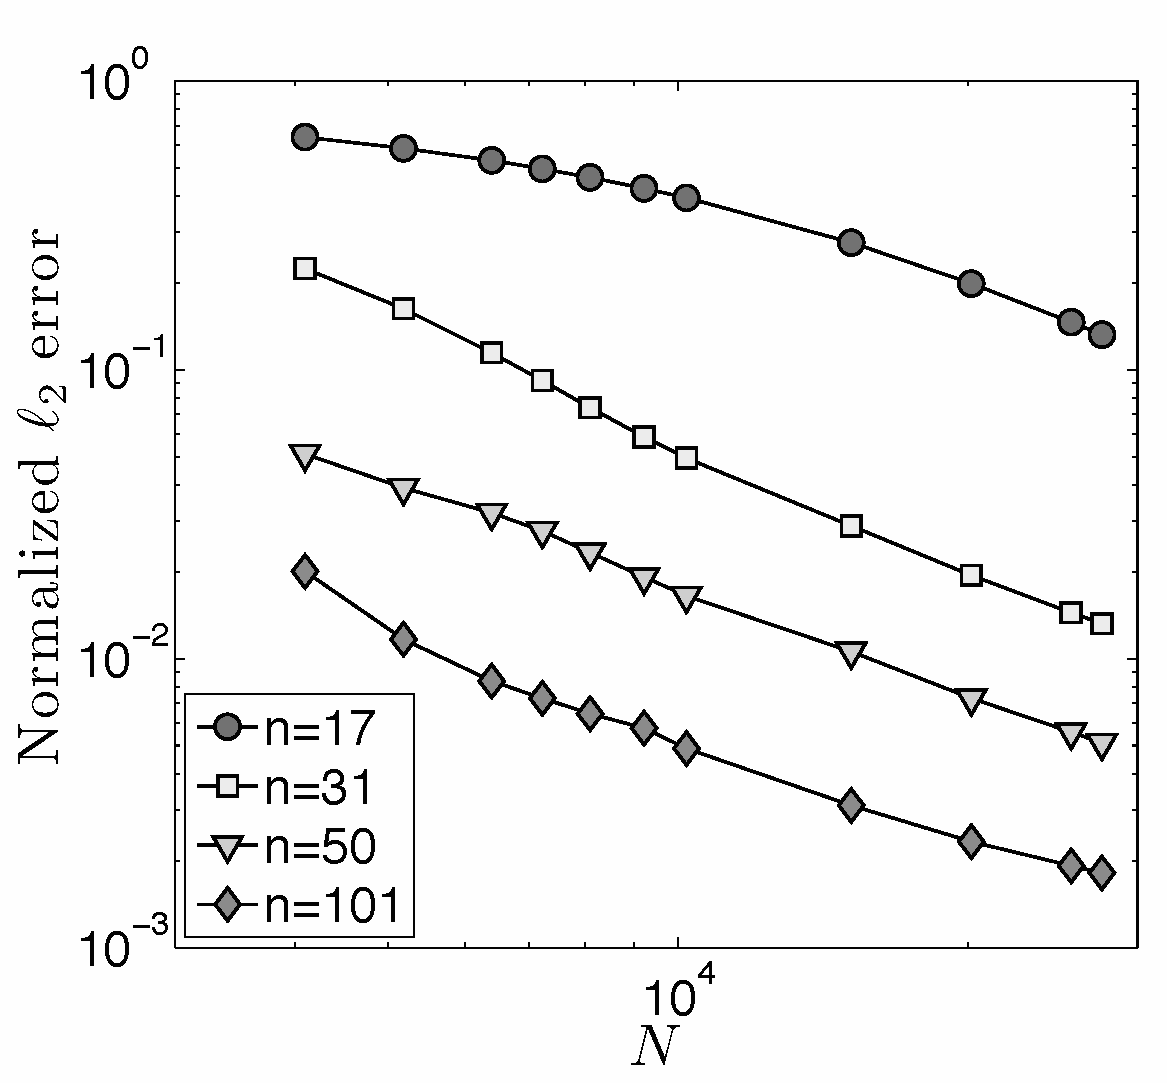
\includegraphics[width=3in]{figures/paper1/figures/cosine_bell/convergence_plot_hv.pdf}
\caption{Convergence plot for cosine bell advection. Normalized $\ell_2$ error at 10 revolutions with hyperviscosity enabled. }
\label{fig:conv_cosine_bell}
\end{center}
\end{figure}


\section{Cut from Paper1}
To verify our multi-CPU and multi-CPU+GPU implementations, two hyperbolic PDEs on the surface of the sphere are tested. For both cases a spherical coordinate system is used in terms of latitude $\lambda$ and longitude $\theta$:
\begin{eqnarray*} 
x & = & \rho \cos \lambda \cos \theta, 	\\
y & = & \rho \sin \lambda \cos \theta, 		\\
z & = & \rho \sin \theta.		
\end{eqnarray*}

Node sets are the Maximum Determinant point distributions on the sphere \cite{Sloan2003} consistent with previously published results (see e.g., \cite{Flyer2007} and \cite{Fornberg2011b}).

Hyperviscosity parameters $\gamma_c$ and $k$ depend on the RHS of the PDE. 
For this test case, hyperviscosity scaling parameters are listed in Table~\ref{tbl:vortex_hv_params}. Linear functions to choose the RBF support parameter $\epsilon$ are also provided. The parameters $\gamma_c$ and $k$ were obtained via trial-and-error parameter searching on $N=4096$ nodes. The goal when choosing parameters is to push all eigenvalues to the left half-plane, and then tweak $\gamma_c$ up or down to condense the eigenvalues as near to the imaginary axis as possible. We try to keep the range of filtered eigenvalue real parts within twice the width of the unfiltered range, so hyperviscosity does not cause too much diffusion in the solution. 

For the cosine bell we use the initial conditions
\begin{equation*}
h  = 
\begin{cases} 
\frac{h_0}{2} (1 + \cos(\frac{\pi \rho}{R})  & \rho \le R  \\
 0 &  \rho \geq R 
\end{cases}
\end{equation*}
where the bell of radius $R = \frac{a}{3}$ is centered at $(\lambda_c, \theta_c)$ and provided by the expression,
\begin{eqnarray*}
\rho = a \arccos( \sin \theta_{c} \sin \theta + \cos \theta_{c} \cos \theta \cos (\lambda - \lambda_{c}) ).
\end{eqnarray*}
We assume $a = 1$, $h_0 = 1$, and $(\lambda_c, \theta_c) = (^{3\pi}/_{2}, 0)$. The angle $\alpha =\ ^{\pi}/_{2}$ is chosen to transport the bell over the poles of the coordinate system, and $u_0 =\ ^{2 \pi a}/_{1036800}$. 

\authnote{Include figures from NCL or Paraview}
